\iffalse
\begin{figure}
    \centering
    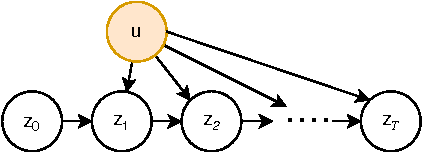
\includegraphics{DAG_ts.drawio.pdf}
    \caption{Directed graphical model for the generating equations \eqref{eq:ts-sem}. }
    \label{fig:ts_dag}
\end{figure}
\fi
\begin{figure}
    \centering
    \begin{tikzpicture}
      % Define nodes
      \node[det]                                (z0)    {$\statest_0$};
      \node[obs, right=of z0 ]               (z1)    {$\state_1$};
      \node[obs, right=of z1 ]               (z2)    {$\state_2$};
      \node[latent, right=of z2 ]               (z3)    {$\state_3$};
      \node[latent, right=of z3 ]               (zt)    {$\ldots$};
      
      \node[latent, above=of z1]            (u)     {$\forcing$};
      
      \edge {u} {z1,z2,z3,zt};
      \edge {z0} {z1};
      \edge {z1} {z2};
      \edge {z2} {z3};
      \edge {z3} {zt};
    \end{tikzpicture} 
    \caption{Bayesian network shown immediately after observation time $t=2$. Shaded circular nodes represent observed nodes. Transparent circular nodes represent unobserved nodes. The diamond initial state $\statest_0$ is known and deterministic. A prior $p(\forcingst)$ is given, as well as the forward operator model~\eqref{eq:ts-sem}, $\state_t = \op{P}(\state_{t-1}, \forcing)$. At this time step, our goal is to compute with an approximation of the posterior of the parameter $\forcing$ given the observations, $p(\forcingst \gvn \state_1 = \statest_1, \state_2=\statest_2)$. More generally, at time step $t$, we are interested in computing with an approximation of the posterior $p(\forcingst \gvn \mathcal{D}_t)$, where $\mathcal{D}_t = \{ \state_1 = \statest_1, \ldots, \state_t=\statest_t\}$.}
    \label{fig:ts_dag}
\end{figure}
